%!TEX root = ../proteoform_suite_manual.tex
%---------------------------------------------------------------------
%	AGGREGATED PROTEOFORMS
%---------------------------------------------------------------------

\section{Aggregated Proteoforms}

\subsection{Overview}

On this page, experimental proteoforms are created by aggregating either raw experimental components (unlabeled analysis) or NeuCode pairs (NeuCode labeled analysis). If Deconvolution Results for Quantification were provided on the Load Results page, these raw experimental components for quantification will be binned with experimental proteoforms based upon the set parameters. The experimental proteoforms are used in intact-mass analysis to identify proteoforms and construct proteoform families.

\subsection{Run Page}
\begin{itemize}
\item The Raw Experimental Components page must be run before running this page. If applicable, the Top-Down and the NeuCode Pairs pages must also be run before running this page.
\item Set all parameters as desired for current analysis (see below)
\item Click Run Page button (top right)
\end{itemize}

\subsection{Set Parameters}
\begin{figure}[h]
\centering
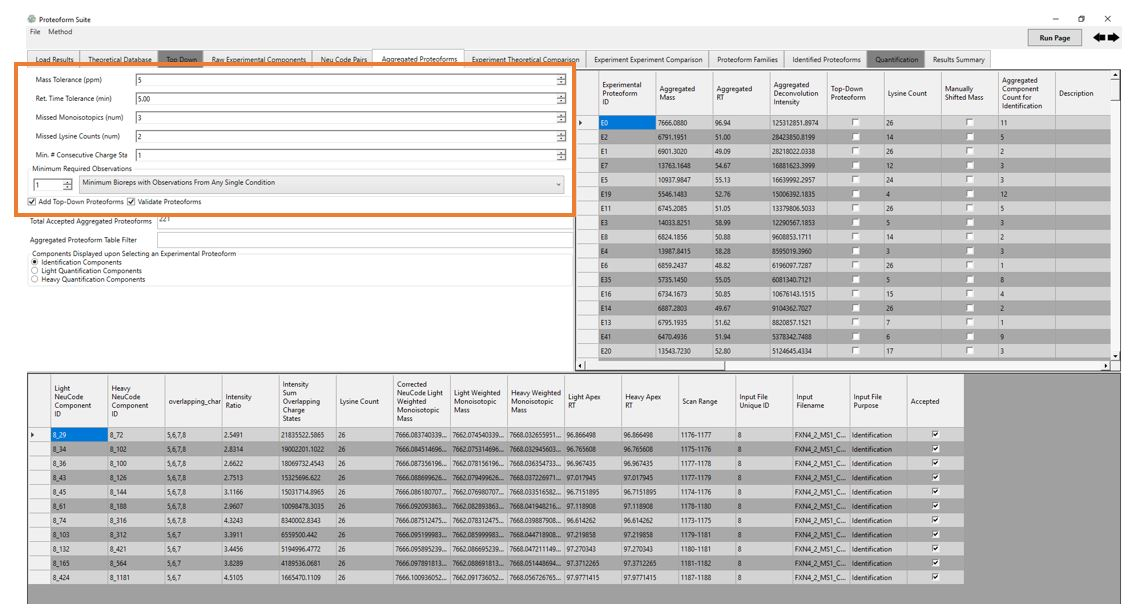
\includegraphics[scale=0.5]{figures/aggregated_proteoforms1.jpg}
\end{figure}
\begin{itemize}
\item Mass Tolerance (ppm): mass tolerance used to aggregate raw experimental components (unlabeled) or NeuCode pairs (NeuCode labeled)
\item Ret. Time Tolerance (min): retention time tolerance used to aggregate raw experimental components (unlabeled) or NeuCode pairs (NeuCode labeled)
\item Missed Monoisotopics (num): number of missed monoisotopic units to aggregate raw experimental components (unlabeled) or NeuCode pairs (NeuCode labeled)
\item Missed Lysine Counts (num): the number of missed lysine counts to aggregate NeuCode pairs (accounts for <100\% labeling efficiency)
\item Min. \# Consecutive Charge States:  minimum number of charge states for a raw experimental component to be considered for aggregation
\item Minimum Required Observations: set the \# (left) and the requirement (right drop down box) to require observations of an experimental proteoform in more than one file type. Must have labeled biological replicates, technical replicates, and conditions for Deconvolution Results for Identification on the Load Results page
\item Add Top-Down Proteoforms: if checked, top-down proteoforms from the Top Down page will be aggregated with experimental proteoforms created from raw experimental components (unlabeled) or NeuCode pairs (NeuCode labeled). Top-down proteoforms will replace experimental proteoforms using the set parameters above
\item Validate Proteoforms: if checked and if NeuCode labeled data, will verify that aggregated NeuCode pairs are in the tolerances determined with set parameters
\end{itemize}

\subsection{Results}
\begin{itemize}
	\item Total Accepted Aggregated Proteoforms: the number of accepted experimental proteoforms that will be included in further analysis
	\item Aggregated Proteoform Table Filter: filter the Aggregated Proteoforms table (top right) by any entered text
	\item Components Displayed Upon Selecting an Experimental Proteoform: determines which components will be displayed in the Components table (bottom) when an aggregated proteoform is selected in the Aggregated Proteoform Table (right)
	\begin{figure}[h]
\centering
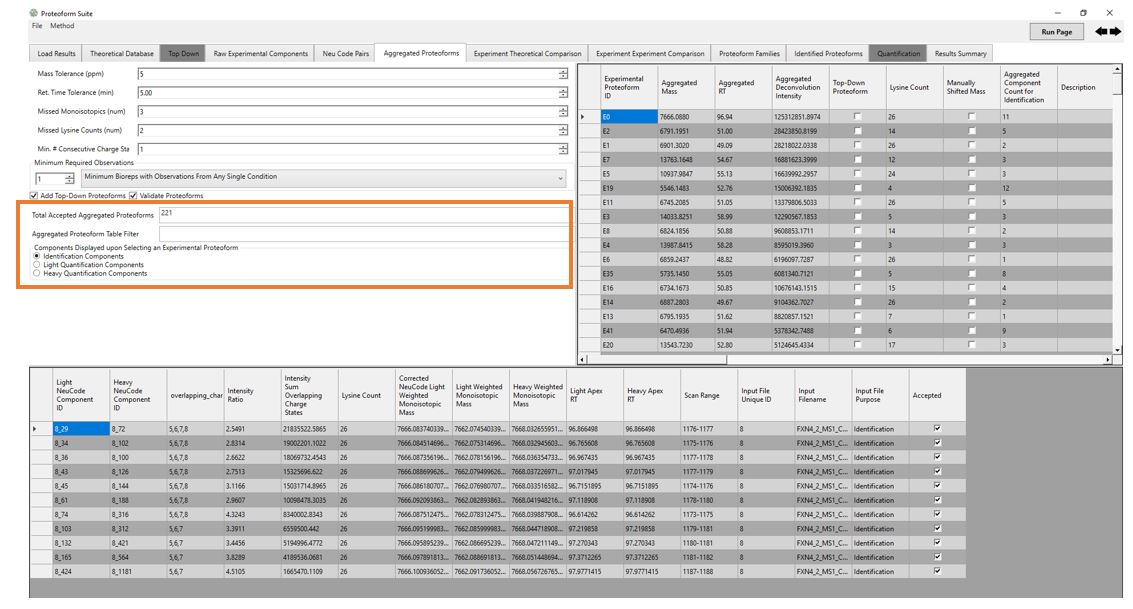
\includegraphics[scale=0.5]{figures/aggregated_proteoforms2.jpg}
\end{figure}
\pagebreak
	\item Aggregated Proteoforms table: the top right table displays the aggregated experimental proteoforms
		\begin{figure}[h]
\centering
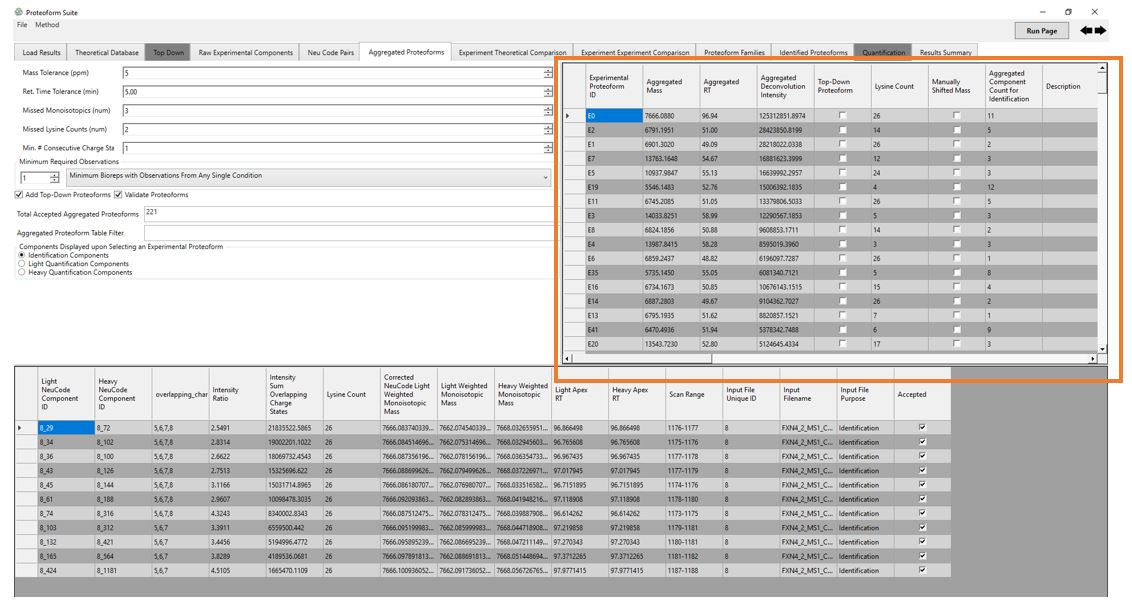
\includegraphics[scale=0.5]{figures/aggregated_proteoforms3.jpg}
\end{figure}
	\begin{itemize}
		\item Experimental Proteoform ID: unique ID given by Proteoform Suite for this experimental proteoform
		\item Aggregated Mass: monoisotopic mass of experimental proteoform, weighted average of (light) raw experimental components by intensity
		\item Aggregated RT: retention time of experimental proteoform, average of raw experimental components (unlabeled) or NeuCode pairs (NeuCode labeled)
		\item Aggregated Deconvolution Intensity: sum of intensity of aggregated raw experimental components
		\item Top-Down Proteoform: checked if this experimental proteoform is a top-down identified proteoform
		\item Lysine Count: number of lysines (NeuCode labeled data)
		\item Manually Shifted Mass: checked if monoisotopic mass was shifted by an isotopic mass unit (see \textbf{Experiment-Theoretical Comparison} section)
		\item Aggregated Component Count for Identification: number of aggregated raw experimental components (unlabeled) or NeuCode pairs (NeuCode labeled). If top-down proteoform, the number of top-down hits
		\item Description: if identified, the protein description from UniProt
		\item Gene Name: if identified, the gene name
		\item GeneID: if identified, the gene ID
		\item Grouped Accessions: if identified, the protein accessions from UniProt
		\item PTM Description: if identified, the post-translational modifications on this experimental proteoform
		\item Begin and End: if identified, the experimental proteoform begin and end residue in protein full sequence in UniProt
		\item Sequence: if identified, proteoform sequence
		\item UniProt-Annotated Modifications: if identified, all UniProt annotated residues for PTMs on this experimental  proteoform in UniProt database provided
		\item Potentially Novel Mods: if identified, checked if this experimental proteoform contains PTMs not annotated in UniProt database provided	
		\item Bottom-Up PSMs Count: if identified, the number of bottom-up PSMs derived from this experimental proteoform
		\item Modified Bottom-Up PSMs: if identified, modified residues confirmed by ID'd bottom-up peptides derived from this experimental proteoform
		\item Bottom-Up Evidence for All PTMs: if identified, checked if all PTMs on this experimental		
		\item Level: proteoform identification level based on five-level scheme\supercite{Smith2019b}
		\item Level Description: description of proteoform level assignment (sources of ambiguity)
		\item New Intact-Mass ID: if identified, this intact-mass identification was not identified by top-down
		\item Ambiguous: checked if ambiguous intact-mass identification
		\item Adduct: checked if identification is due to presence of an adduct (oxidation, SDS adduct, sulfate adduct)
		\item Contaminant: checked if identification is from a theoretical proteoform in a contaminant database
		\item Mass Error: mass difference between observed mass and theoretical mass of this identification
		\item Family ID: proteoform family number (must have run through full Proteoform Suite analysis)
		\item Family: identified, ambiguous, or unidentified proteoform family
		\item Linked Proteoform References: proteoforms in family network path of identification to the nearest theoretical proteoform (must have run through full Proteoform Suite analysis)
		\item M/z values: m/z values observed for this experimental proteoform
		\item Charges: charge state numbers observed for this experimental proteoform
		\item Abundant Component for Manual Validation of Identification: file information for the most abundant raw experimental component aggregated into this experimental proteoform
	\end{itemize}
	\item Components table: the bottom table displays all raw experimental components (unlabeled) or NeuCode pairs (NeuCode labeled) aggregated into the experimental proteoform selected in the Aggregated Proteoforms table (top right)
		\begin{figure}[h]
\centering
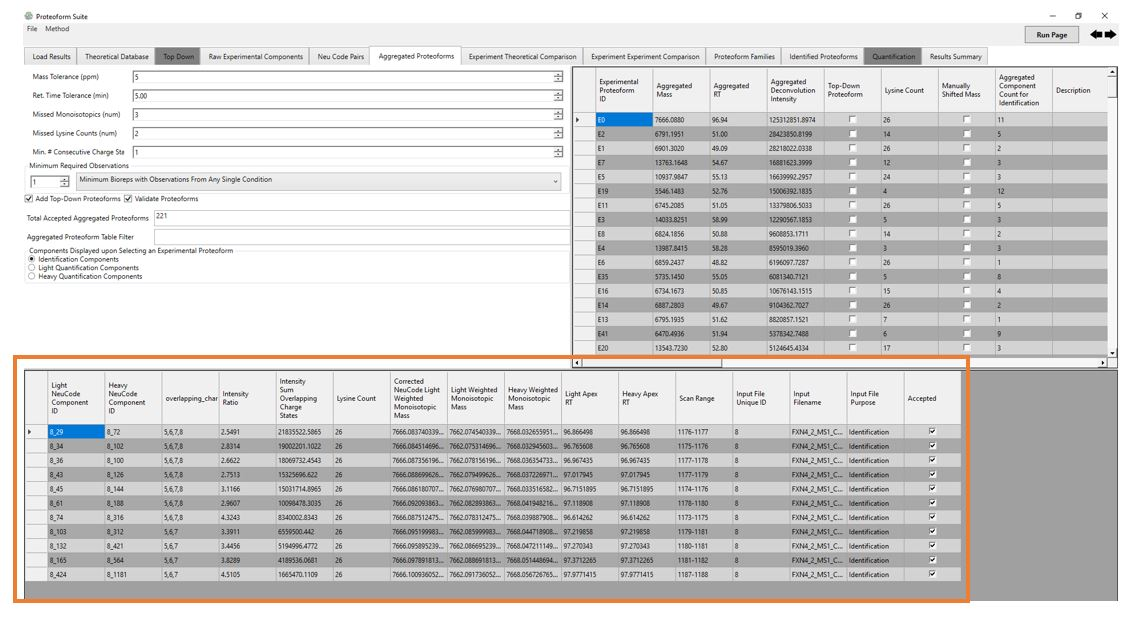
\includegraphics[scale=0.5]{figures/aggregated_proteoforms4.jpg}
\end{figure}
	\begin{itemize}
		\item See Raw Experimental Components table in \textbf{Raw Experimental Components} section (unlabeled) or NeuCode Pairs table in \textbf{NeuCode Pairs} section (NeuCode labeled) for a description of each column
	\end{itemize}
\end{itemize}